% !TEX root = main.tex

\section{中文词法分析}
\subsection{基本概念}
\begin{definition}[词]
能够独立运用的最小音义结合体。
\end{definition}

若$S$是一个词,则满足
\begin{itemize}
\item $S$内部字串粘合度高
\item $S$外部环境替换度高
\item $S$本身频度高
\end{itemize}

\subsection{文本分词中的歧义}
\begin{itemize}
	\item 交集性歧义
\begin{displayquote}
大学生$\mid$不看重$\mid$大城市$\mid$户口\\
大学生$\mid$不看$\mid$重大城市$\mid$户口\\
\end{displayquote}
	\item 组合型歧义
\begin{displayquote}
你认为学生会$\mid$听老师的吗\\
你认为学生$\mid$会听老师的吗\\
\end{displayquote}
\end{itemize}

\subsection{基本方法}
\[\text{中文分词方法}\begin{cases}
\text{基于词典的分词方法}\begin{cases}
\text{最大匹配法}\\
\text{最短路径法}\\
\text{半词罚分法}\\
\text{最大概率法}
\end{cases} & \text{分词}\\
\text{基于子序列标注的方法}\begin{cases}
\text{最大熵模型}\\
\text{CRF模型}
\end{cases} & \text{合词}
\end{cases}\]

\subsubsection{最大匹配法}
最大匹配法:有一个词典,设定最大词长,做字符串匹配
\begin{figure}[H]
\centering
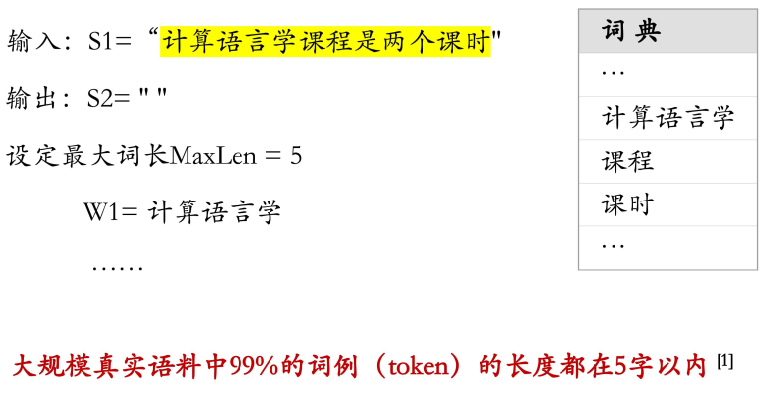
\includegraphics[width=0.6\linewidth]{fig/max_matching.png}
\end{figure}

\subsubsection{最优路径法}
\begin{itemize}
\item 最短路径法:词数最少最优
\item 半词罚分法(加权):如果一个字不能单独使用则是半词,每个词罚1分,每个半词加罚1分,求罚分最低路径
\item 最大概率法:在词图上选择词串概率最大的分词路径(动态规划),最优路径中第$i$个词$W_i$的累积概率等于左邻词$W_{i-1}$累积乘自身
\[P'(w_i)=P'(w_{i-1})\times P(w_i)\]
为方便计算,通常将概率转为路径代价,即取对数。
\begin{enumerate}
	\item 对一个待分词的字串$S$,按照从左到右的顺序取出全部候选词$w_1,\ldots,w_i,\ldots,w_n$
	\item 到词典中查出每个候选词的概率值$P(w_i)$,转换为代价$C(w_i)$,并记录每个候选词的全部左邻词
	\item 按照$C'(w_i)=C'(w_{i-1})+C(w_i)$计算累计代价,同时比较得到每个候选词的最佳左邻词
	\item 如果当前$w_n$是字串$S$的尾词,且累积代价$C'(w_n)$最大,则$w_n$即为$S$的终点词
	\item 从$w_n$开始,从右到左依次将最佳左邻词输出,即为$S$的分词结果
\end{enumerate}
\end{itemize}
\begin{figure}[H]
\centering
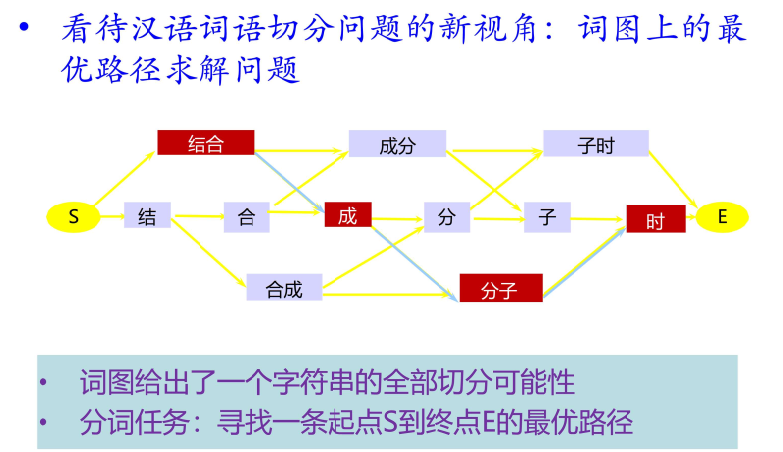
\includegraphics[width=0.6\linewidth]{fig/best_path.png}
\end{figure}

\subsubsection{基于字序列标注的方法}
字位标注法:分词可以看作是对字加``词位标注''的过程。
根据字本身及其上下文特征来决定当前字的词位标注。
\begin{figure}[H]
\centering
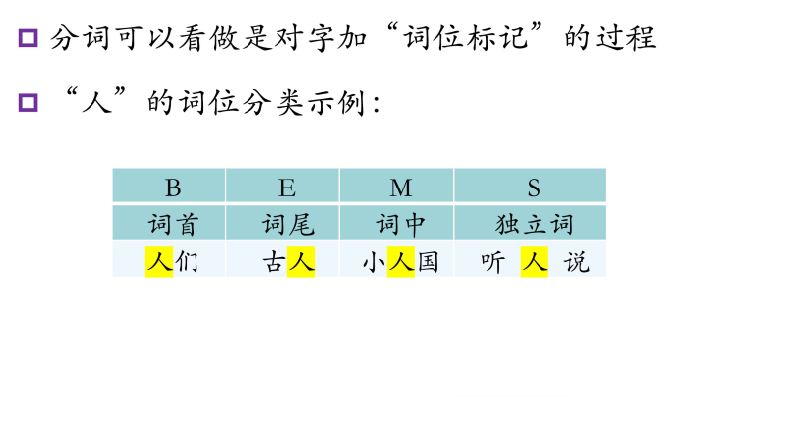
\includegraphics[width=0.6\linewidth]{fig/word_pos_labeling.png}
\end{figure}

\subsubsection{评价指标}
\[\begin{aligned}
\text{准确率}P=\frac{\#切分正确}{\#切分结果所有分词}\\
\text{召回率}R=\frac{\#切分正确}{\#标准答案所有分词}\\
\text{F评价}F_1=\frac{2PR}{P+R}
\end{aligned}\]